\section{Sensorer}
Dette afsnit vil undersøge de sensorer der er interessante for dette projekt.
Der vil blive beskrevet de forsøg der er blevet udført, for at teste deres nøjagtighed og komme med en konklusion på hvor nøjagtige de er.
Disse forsøg vil samtidig blive holdt op imod de forsøg der er blevet udført i \cite{tikNXT}, på de samme sensorer.

\subsection{Ultrasonic Sensor}
Ultrasonic sensoren(US), som kan ses på \cref{sensor:ultrasonic_sensor}, er en sensor der kan måle afstande til objekter.

\begin{figure}[h]
\centering
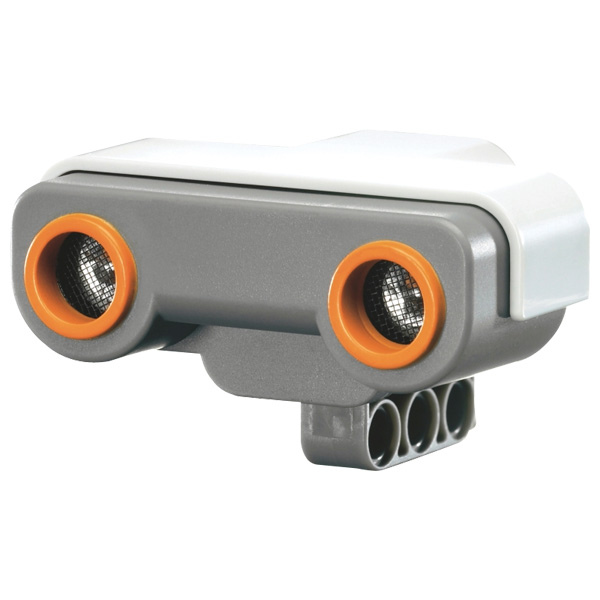
\includegraphics[width=.5\textwidth]{us}
\caption{\legoms Ultrasonic Sensor}
\label{sensor:ultrasonic_sensor}
\end{figure}

Dette gøres ved at der sendes en lydbølge, hvorefter der så beregnes hvor lang tid det tager for denne at ramme objektet og så komme tilbage igen.
US'en måler afstanden i cm eller tommer og den maksimale aftsand der kan måles er 255 cm, med en præcision på $\pm$3 centimeter.\cite{tikNXT}

\paragraph{Eksperimenterne} foretaget i \cite{tikNXT} har vist at
\begin{itemize}
\item den minimale aftsand der kan måles er 3 cm.
\item det bedst genkendelig objekt et objekt der har glat og hård overflade og som er firkantet.
\item desto mindre objektet er, desto sværere har sensoren ved at se objektet.
\item sensorens højre 'øje' er det der sender lydbølgen, mens det venstre modtager.
Det gør at US'en 'ser' bedre i højre side når sensoren befinder sig i horisontal position.
Dette kan tydelig ses når afstand mellem sensor og objekt er under 20 cm, da den slet ikke kommer i sensorens venstre synsfelt.
\item hvis sensoren anvendes i vertikal position er der det problem at modtagelsen af bølgerne kan blive distraheret af underlaget.
\end{itemize}

\paragraph{Den bedste opstilling} for US'en er i horisontal position, der opnås de bedste resultater, fordi den kritiske region ifht. den vertikale position er mindre.
En vinkel på mere end 15 grader fra lydbølgen giver hellere ikke klare resultater.
Desuden er runde genstande også svært genkendelige for US'ens synsfelt.

\subsubsection{Test}
Der er gennemført en mindre test af US'en, for at svare på følgende spørgsmål:

\begin{itemize}
\item Hvor langt rækker US'en i praksis?
\item Hvor stor nøjagtighed har den i praksis?
\item Ligner resultaterne dem fra eksperimenterne ovenfor?
\end{itemize}

\paragraph{Opstillingen} som blev brugt til at svare på disse spørgsmål kan ses i \cref{sensor:ultrasonic_opstilling}, bestående af: tommestok, NXT 2.0, \legoms Ultrasonic Sensor og \legoms kabel.
Tommestokken blev brugt til at måle den nøjagtige afstand og derefter blev sensoren aflæst.
\mikael{Er det vigtigt med et billede af opstillingen? Er det ikke nok bare at beskrive den?}
\bruno{skal evt. i appendix}

\begin{figure}[h]
\centering
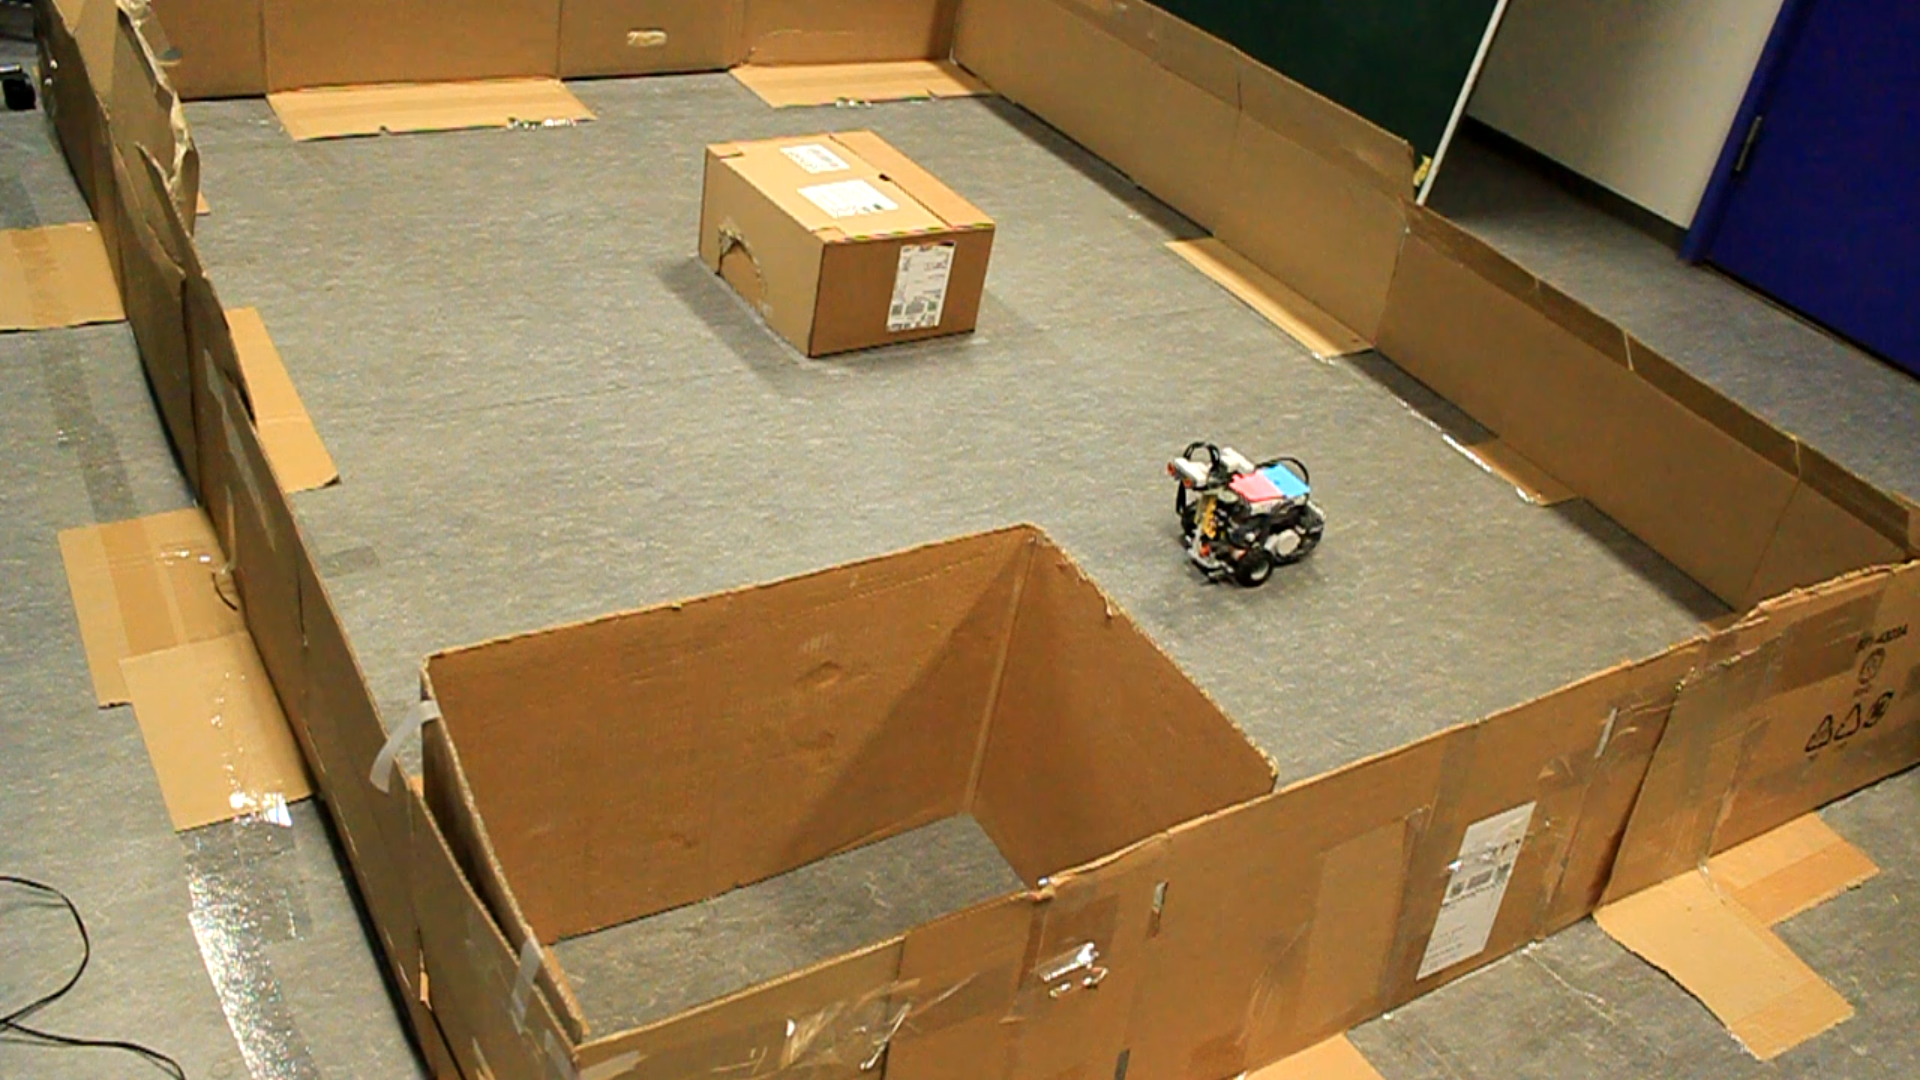
\includegraphics[width=.75\textwidth]{opstilling}
\caption{Forsøgsopstilling for test af US'ens afstands præcision}
\label{sensor:ultrasonic_opstilling}
\end{figure}

\begin{figure}[h]
\centering
\begin{tabular}{r | c | c | c |}
optimal & test1 & test2 & test3 \\
\hline
1 & 6 & 6 & 6 \\
10&	22&	23&	23\\
20&	22&	23&	23\\
30&	31&	31&	32\\
40&	40&	41&	40\\
50&	50&	50&	51\\
60&	60&	61&	61\\
70&	70&	71&	66\\
80&	80&	81&	81\\
90&	90&	91&	91\\
100&	100&	101&	102\\
110&	111&	112&	112\\
120&	120&	121&	121\\
130&	131&	131&	131\\
140&	141&	141&	141\\
150&	151&	151&	151\\
160&	161&	161&	163\\
170&	171&	171&	171\\
180&	255&	181&	181\\
190&	255&	190&	191\\
200&	202&	201&	202\\
210&	255&	255&	213\\
220&	255&	255&	222\\
230&	255&	255&	232\\
240&	255&	255&	255\\
250&	255&	255&	255\\
260&	255&	255&	255\\
\end{tabular}
\caption{Forsøgsresultater: afstande til objekt i cm.}
\label{sensor:ultrasonic_test_data}
\end{figure}

\paragraph{Resultaterne} fra forsøget kan ses i \cref{sensor:ultrasonic_test_data}.
I \cref{sensor:ultrasonic_resultat_diagram} kan det ses hvordan at de tre tests alle giver forkerte resultater når US'en er mindre en 20 cm fra objektet.
Desuden kan det ses på \cref{sensor:ultrasonic_resultat_diagram} at der i test1 kun kunne måles op til 170 cm før der opstod usikkerhed, men de andre tests nåede 200(test2) og 230(test3) cm før der opstod større usikkerhed.
Generelt holder det som der bliver lovet, nemlig at der er en afvigelse på 3 cm på målingerne, men forsøget viser at der kun med sikkerhed kan måles mellem 20 og 170 cm.

\begin{figure}[h]
\centering
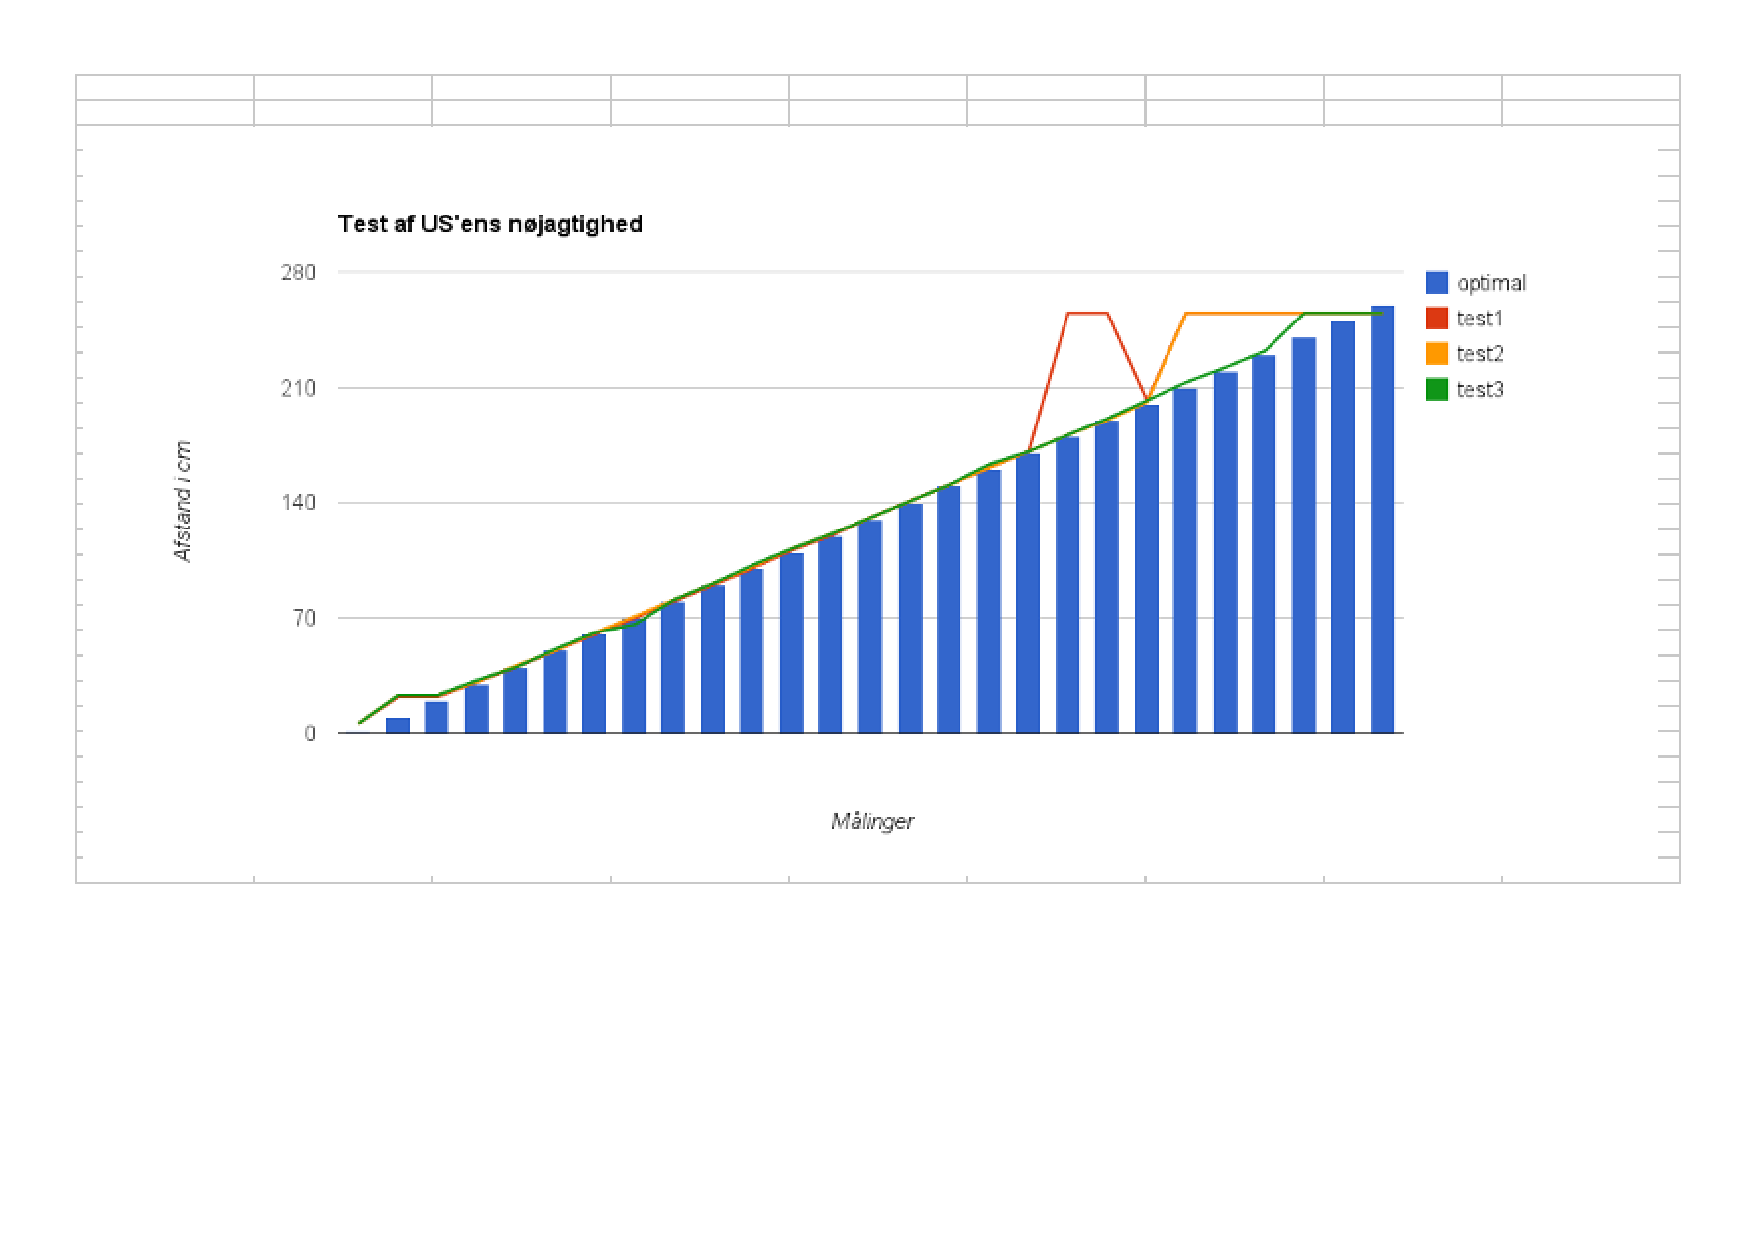
\includegraphics[width=\textwidth]{us_result_diagram}
\caption{Testresultater: De blå søjler repræsenterer den målte afstand med tommestok, de andre tre viser US'ens testresultater ifht. hianden.}
\label{sensor:ultrasonic_resultat_diagram}
\end{figure}


\subsection{Infarød Sensor}
Den infarøde afstandssensor(IS) som kan ses på \ref{sensor:infraroed_sensor} er en afstandssensor med høj præcision og et interval på 10 til 80 cm.
\bruno{sensor not working at the moment :i}

\begin{figure}[h]
\centering
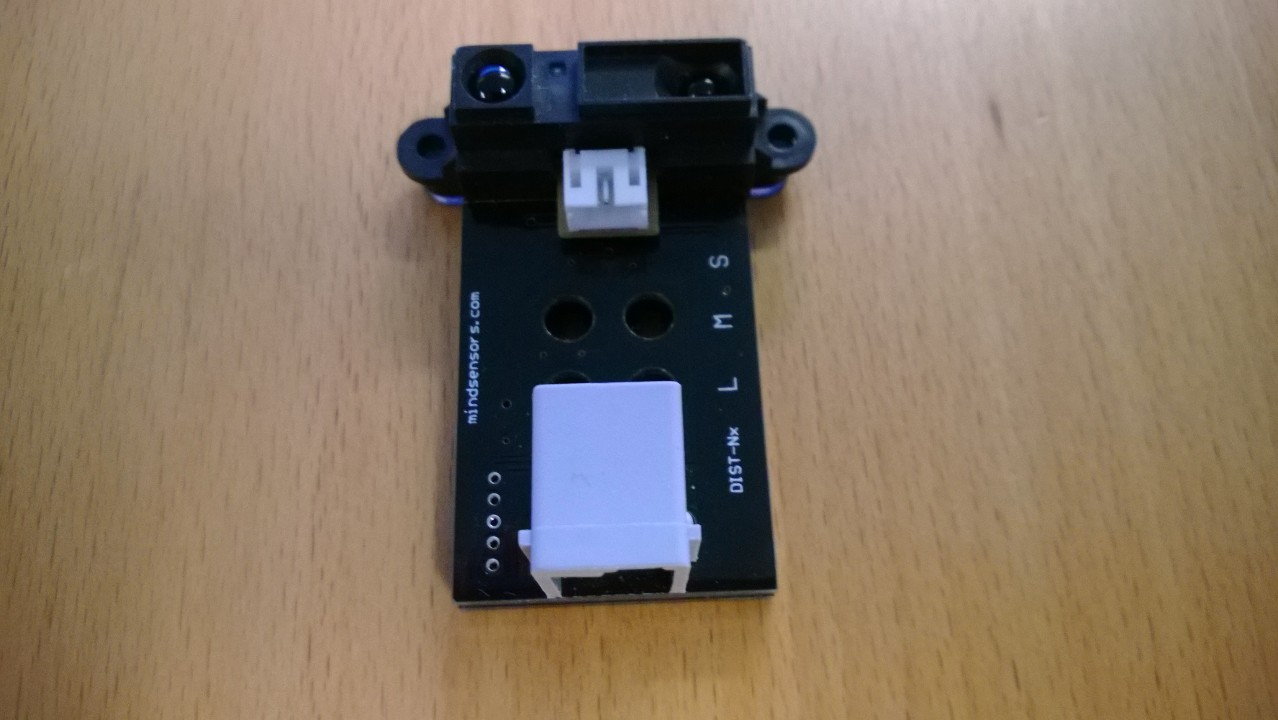
\includegraphics[width=.5\textwidth]{is} 	
\caption{High Precision Medium Range Infrared Distance Sensor for NXT (v2)}
\label{sensor:infraroed_sensor}
\end{figure}

\subsection{Motor}
Motoren som dette afsnit handler om er en el-motor som er \lego's egen.
Motoren består af en rotationssensor som måler omdrejningerne ved grader, denne har en nøjagtighed på 1 grad. Det er med til at gøre motoren ret præcis. 
Desuden gør denne sensor det også muligt at styre, hvor meget kraft mortoren skal køre med.
Hvis man kører med flere motorer så har NXT'en indbygget software der gør det muligt at synkronisere disse motorer.
Det er smart hvis den ene motor skulle være stærkere eller svagere end den anden.\cite{tikNXT}
Motoren kan ses på figur \ref{sensor:motor_sensor}.
\\

\begin{figure}[h]
\centering
%http://www.philohome.com/nxtmotor/nxtmotor.htm
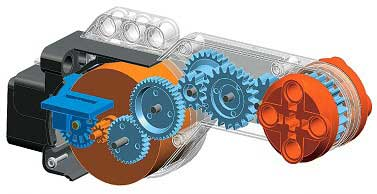
\includegraphics[width=.5\textwidth]{motor} 	
\caption{\legoms Servo Motor}
\label{sensor:motor_sensor}
\end{figure}

\paragraph{Eksperimenterne} i \cite{tikNXT} har vist at
\begin{itemize}
\item ved forsøg med en TriBot hvor den skal gøre samme vej tilbage som den kom fra, rammer den flere centimeter ved siden af.
\item antallet af centimeter den afviger i førnævnte punkt stiger med afstanden og omvendt.
\item der er konstateret en afvigelse på $\pm$2 grader, som fortæller os hvorfor den store afvigelse i centimeter i TriBot forsøget.
\item selvom den indbyggede rotationssensor har motorerne ikke stor præcision.
\end{itemize}

\subsubsection{Test}
Der er gennemført en test af motoren, for at svare på følgende spørgsmål:

\begin{itemize}
\item Kan det virkelig passe at den har 1 grads nøjagtighed?
\item Hvad er den praktiske nøjagtighed?
\item Giver motorerne det samme resultat når de er synkroniserede?
\end{itemize}

\paragraph{Opstillingen} brugt for at svare på disse spørgsmål, kan ses i figur \ref{sensor:motor_sensor_opstilling}.
\mikael{Er det nødvendigt at vise opstillingen? Er det ikke nok bare at beskrive den?}

\begin{figure}[h]
\centering
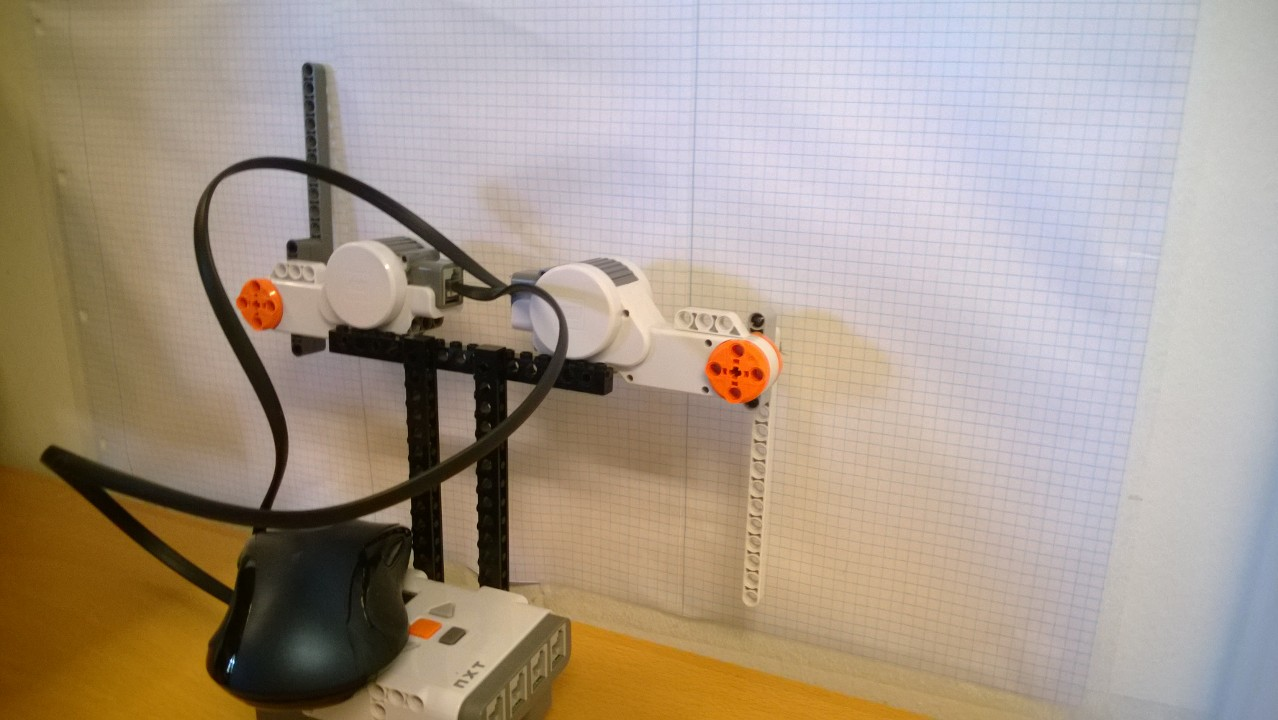
\includegraphics[width=.75\textwidth]{motor_opstilling} 	
\caption{Forsøgsopstillingen for motor nøjagtighedstesten.}
\label{sensor:motor_sensor_opstilling}
\end{figure}

Forsøgsopstillingen består af følgende dele:
\begin{itemize}
\item NXT v2
\item 2x \legoms motor sensor
\item 2x \legoms kabler
\item Lidt \lego til at bygge holderen til motorerne og en forlænger til motorerne for letter måling.
\item 3 A4 ark(ternet)
\item Tape
\item Vinkelmåler
\item Stiftblyant
\end{itemize}

Sådan blev forsøget gennemført:

\begin{enumerate}
\item Der startes med at bygge et stativ til de to motorer på NXT'en.
\item Derefter sættes de to motorer på stativet og forbindes vha. kablerne til NXT'en.(Her er der brugt noget modvægt, så NXT'en ikke vælter, musen på figur \ref{sensor:motor_sensor_opstilling}).
\item De tre A4 ark sættes op på en væg, vha. tape, så midten af papiret passer med de to motorers højde.
\item Der sættes nu en forlænger på de to motorer, så det passer med at forlængeren holder sig over papiret på en omdrejning.
\item Afmærk midten af motoren på papiret vha. at sætte en stiftblyant igennem midten af motorens akse.
\item Sæt motoren igang og afmærk hvor forlængeren stopper.
\item Det afmærkede midter punkt bliver brugt til at måle vinklen, til det afmærkede punkt udenfor forlængeren, vha. vinkelmåleren.
\item Desuden noteres tacho-værdien(antal grader drejet) som kan trækkes ud fra motorens rotationssensor vha. software.
\end{enumerate}

\begin{figure}[h]
\centering
\begin{tabular}{r | c | c | c | c | r |}
grader sat & \parbox{2.5cm}{motor b \\ grader målt*} & \parbox{2.cm}{motor b \\ tacho slut**} &  \parbox{2.5cm}{motor b \\ grader målt*} & \parbox{2.5cm}{motor b \\ tacho slut**} & optimal \\
\hline
1&	1&	0&	1&	0&	1\\
2&	2&	2&	2.5&	2&	2\\
3&	2&	3&	3&	3&	3\\
4&	5&	4&	4&	3&	4\\
5&	5&	6&	4&	4&	5\\
10&	10&	9&	9&	10&	10\\
15&	11&	16&	14&	15&	15\\
20&	20&	20&	18&	20&	20\\
25&	21&	25&	23&	25&	25\\
50&	57&	50&	56&	50&	50\\
75&	80&	77&	80&	79&	75\\
100&	100&	99&	95&	100&	100\\
150&	150&	149&	145&	150&	150\\
200&	204&	197&	200&	199&	200\\
400&	400&	401&	400&	398&	400\\
800&	799&	800&	800&	799&	800\\
1200&	1204&	1201&	1200&	1200&	1200\\
1800&	1796&	1796&	1799&	1800&	1800\\
3600&	3601&	3600&	3597&	3599&	3600\\

\end{tabular}
\caption{Forsøgsresultater for motor nøjagtighedstesten.}
\label{sensor:motor_test_data}
\end{figure}

\paragraph{Resultaterne} fra forsøget kan ses i \cref{sensor:motor_test_data}.
Hvis vi kigger på figur \ref{sensor:motor_test_data} så kan vi se at den største afvigelse er +7 grader målt og -4 grader målt.
Tacho-værdien har en afvigelse på maksimalt +1 og -4 grader.
Dette stemmer ikke overens med de antagede $\pm$1 grad afvigelse.

+7 og +6 grader målt optræder kun en gang ellers er den maksimale målte afvigelse $\pm$4 grader, men selvom vi antager at det er pga. unøjagtige målinger ved forsøgsudførelsen er det stadig ikke $\pm$1 grad.

Hvis vi kigger på figur \ref{sensor:motor_sensor_diagram1}
kan vi se at de målte målinger ligger længst udenfor optimalen(sorte stiplede linje).
Det vil sige tacho-værdien er bedre at gå efter.

Desuden kan vi se på samme figur at motor b er meget mere unøjagtig end motor c.
Ideelt ville de to motorer give det samme resultat.

Dvs. den målte værdi har en afvigelse på $\pm$4, mens tacho-værdien har en afvigelse på +1 og -4, og at synkronisering af de to motrer ikke giver den ønskede effekt.

\begin{figure}[h]
\centering
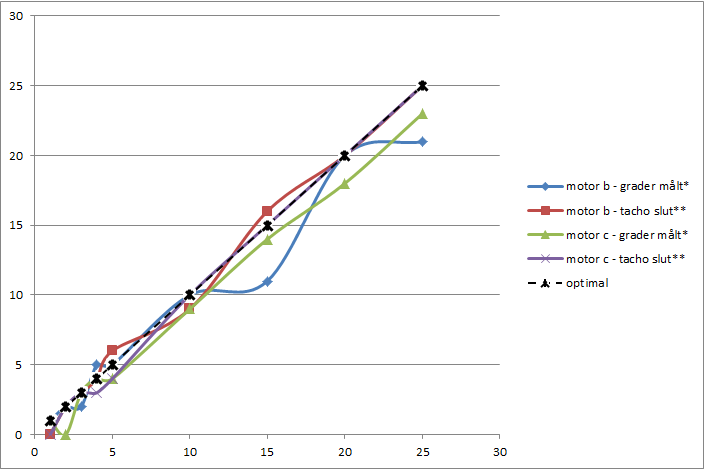
\includegraphics[width=.75\textwidth]{motor_diagram1} 	
\caption{Forsøgsdiagram for forsøget omkring motorens nøjagtighed, grader 0 til 50.}
\label{sensor:motor_sensor_diagram1}
\end{figure}

\begin{figure}[h]
\centering
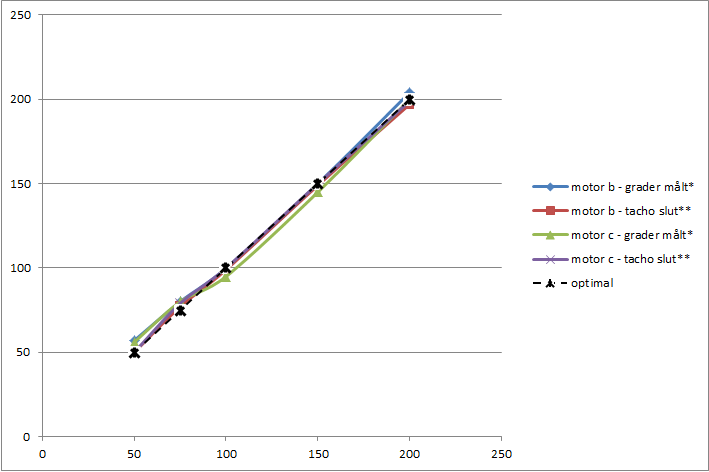
\includegraphics[width=.75\textwidth]{motor_diagram2} 	
\caption{Forsøgsdiagram for forsøget omkring motorens nøjagtighed, grader 50 til 200.}
\label{sensor:motor_sensor_diagram2}
\bruno{Ikke brugt i teksten, kan være den bare skal smides ud}
\end{figure}

\begin{figure}[h]
\centering
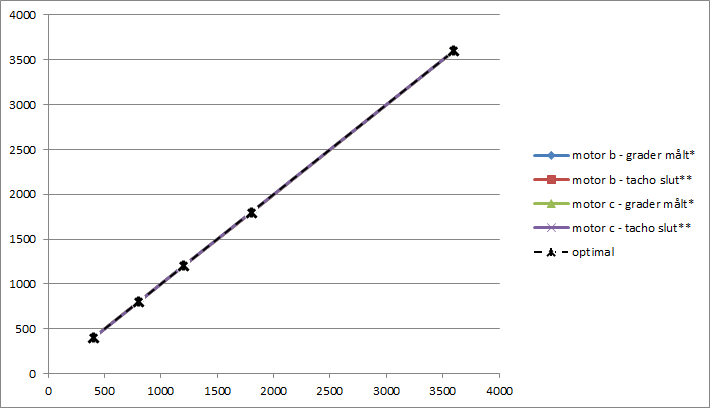
\includegraphics[width=.75\textwidth]{motor_diagram3} 	
\caption{Forsøgsdiagram for forsøget omkring motorens nøjagtighed, grader 200 til 3600.}
\label{sensor:motor_sensor_diagram3}
\bruno{Ikke brugt i teksten, kan være den bare skal smides ud}
\end{figure}